\documentclass{article}
\usepackage{tikz}
\usepackage{biblatex}
\usepackage{caption}
\addbibresource{T2000-1.bib}

\begin{document}
\begin{figure}
\centering

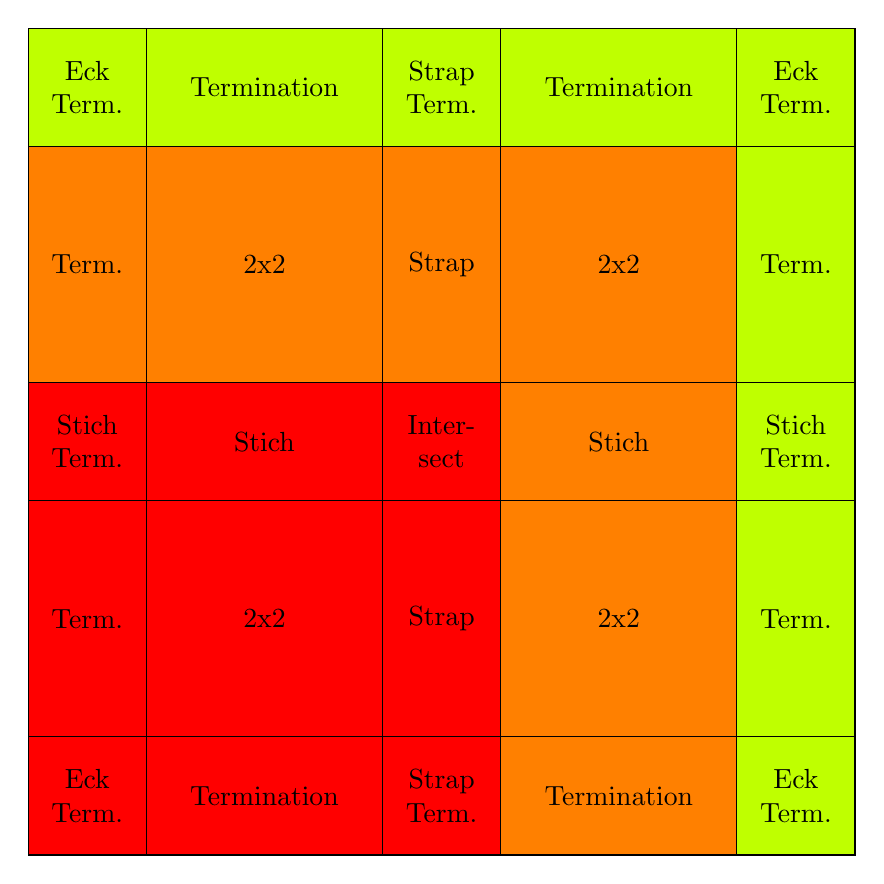
\begin{tikzpicture}[scale= 1.5]
	\filldraw[draw=black, fill = red] (0,0) rectangle (1,1) node[pos=.5, text width = 1cm, align=center] {Eck \linebreak Term.};
	\filldraw[draw=black, fill = red] (0,1) rectangle (1,3) node[pos=.5] {Term.};
	\filldraw[draw=black, fill = red] (0,3) rectangle (1,4) node[pos=.5, text width = 1cm, align=center] {Stich \linebreak Term.};
	\filldraw[draw=black, fill = orange] (0,4) rectangle (1,6) node[pos=.5] {Term.};
	\filldraw[draw=black, fill = lime] (0,6) rectangle (1,7) node[pos=.5, text width = 1cm, align=center] {Eck \linebreak Term.};
	
	\filldraw[draw=black, fill=red] (1,0) rectangle (3,1) node[pos=.5] {Termination};
	\filldraw[draw=black, fill=red] (1,1) rectangle (3,3) node[pos=.5] {2x2};
	\filldraw[draw=black, fill=red] (1,3) rectangle (3,4) node[pos=.5] {Stich};
	\filldraw[draw=black, fill=orange] (1,4) rectangle (3,6) node[pos=.5] {2x2};
	\filldraw[draw=black, fill=lime] (1,6) rectangle (3,7) node[pos=.5] {Termination};
	
	\filldraw[draw=black, fill=red] (3,0) rectangle (4,1) node[pos=.5, text width = 1cm, align=center] {Strap \linebreak Term.};
	\filldraw[draw=black, fill=red] (3,1) rectangle (4,3) node[pos=.5] {Strap};
	\filldraw[draw=black, fill=red] (3,3) rectangle (4,4) node[pos=.5, text width = 1cm, align=center] {Inter-\linebreak sect};
	\filldraw[draw=black, fill=orange] (3,4) rectangle (4,6) node[pos=.5] {Strap};
	\filldraw[draw=black, fill=lime] (3,6) rectangle (4,7) node[pos=.5, text width = 1cm, align=center] {Strap \linebreak Term.};
	
	\filldraw[draw=black, fill=orange] (4,0) rectangle (6,1) node[pos=.5] {Termination};
	\filldraw[draw=black, fill=orange] (4,1) rectangle (6,3) node[pos=.5] {2x2};
	\filldraw[draw=black, fill=orange] (4,3) rectangle (6,4) node[pos=.5] {Stich};
	\filldraw[draw=black, fill=orange] (4,4) rectangle (6,6) node[pos=.5] {2x2};
	\filldraw[draw=black, fill=lime] (4,6) rectangle (6,7) node[pos=.5] {Termination};
	
	\filldraw[draw=black, fill = lime] (6,0) rectangle (7,1) node[pos=.5, text width = 1cm, align=center] {Eck \linebreak Term.};
	\filldraw[draw=black, fill = lime] (6,1) rectangle (7,3) node[pos=.5] {Term.};
	\filldraw[draw=black, fill = lime] (6,3) rectangle (7,4) node[pos=.5, text width = 1cm, align=center] {Stich \linebreak Term.};
	\filldraw[draw=black, fill = lime] (6,4) rectangle (7,6) node[pos=.5] {Term.};
	\filldraw[draw=black, fill = lime] (6,6) rectangle (7,7) node[pos=.5, text width = 1cm, align=center] {Eck \linebreak Term.};

\end{tikzpicture}
\captionsetup{singlelinecheck=off}
\caption{Schematische Zellanordnung entsprechend der Konvention\\
Rot: Diese Zellen müssen in der richtigen Orientierung vorliegen\\
Orange: Diese Zellen liegen bei Beachtung der Roten Zellen automatisch in der richtigen Orientierung vor\\
 Grün: Diese Zellen werden vom Programm gedreht}
\label{figure:aufbau_farb}
\end{figure}

\nocite{*}
\printbibliography{}
\end{document}